\documentclass[a4paper,11pt]{kth-mag}
\usepackage[T1]{fontenc}
\usepackage{textcomp}
\usepackage{lmodern}
\usepackage[utf8]{inputenc}
\usepackage[swedish,english]{babel}
\usepackage{modifications}
\usepackage{framed}
\usepackage{graphicx}
\usepackage{url}
\title{Voting Mix-Net}
% Bibliograhpy -> References
\addto\captionsenglish{
\renewcommand\bibname{References}
}

\subtitle{Implementing a mix-net for use in electronic voting systems}
\foreigntitle{Mix-nät för röstning}
\author{Joakim Uddholm Hjalmarsson}
\date{April 2013}
\blurb{Bachelor's Thesis at NADA\\Supervisor: Douglas Wikström\\Examiner: Mårten Björkman}
\begin{document}
\frontmatter
\pagestyle{empty}
\removepagenumbers
\trita{}
\maketitle
\selectlanguage{english}
\begin{abstract}
In this report I present a partial implementation of the mix-net protocol described by Khazaei, Moran and Wikström in "A Mix-Net From Any CCA2 Secure Cryptosystem" for use in electronic voting. The report goes into detail how the different components of the mix-net work and how the voting system works. The implementation is not complete, but is seen as a good start towards what could become a secure electronic voting system.
\end{abstract}
\clearpage

\begin{foreignabstract}{swedish}
I denna rapport presenterar jag en partiellt genomförande av protokollet som beskrivs av Khazaei, Moran och Wikström i rapporten "A Mix-Net From Any CCA2 Secure Cryptosystem" för användning i elektronisk röstning. Den här rapporten går in på detaljer om hur de olika komponenterna i mix-nätets implementationen och röstningssystemet fungerar. Implementationen anses inte vara fullständig, men ses som en bra start mot vad som kan bli ett säkert elektroniskt röstningssystem.
\end{foreignabstract}
\clearpage
\tableofcontents*
\mainmatter
%\pagestyle{newchap}

\chapter{Introduction}
Many of todays electronic voting system are implemented using mix-nets or mix networks, a term first introduced by David Chaum \cite{1}. The goal of a mix network, abbreviated as mix-net, is to hide correspondence between an input and an output, and was originally intended to be used for anonymous emailing. Todays examples of other applications which use mix-nets can, but is not limited to include anonymous web browsing such as the Tor project\cite{2} as well as in payment systems\cite{3}.

The basic decryption mix-net works as a chain of proxy servers, each with its own public and private key. In this report the proxy server will be henceforth be called a mix-server. The client encrypts its input once using each of the proxy servers’ public key in a certain order. The mix-servers then decrypts the input in that same order. Each mix-server takes a list of encrypted texts. It decrypts them using its private key, shuffles the order and then sends it to the next mix-server.

This method ensures that each mix-server has to be part of the decryption process. However, certain vulnerabilities still present themselves in this basic model. For example, if the last server is corrupt, it could tamper with the plaintext result since it will do the last decryption step.

In this report I describe an implementation of a mix-net as well as a basic voting system built on top of it. I look at the performance of a small sample election and the general feasibility of implementing voting systems using mix-nets. 

\chapter{Background}
\section{Related Work}
There are a numerous amount of commercial electronic voting systems available as well as controversy surrounding them. For example in 2004 an electronic voting system made by Diebold used in the U.S. elections was found to be vulnerable to a number of different attacks [5]. This shows the need for secure voting systems. There are also open source voting systems, such as Helios\cite{10} and Scantegrity\cite{11}.  Helios is a web based voting system served via HTTP to be used for smaller elections while Scantegrity is an enhancement for (physical) optical scan voting system. Both systems provide end-to-end auditability, providing users with a method to track their votes. Another electronic voting system is Prêt-à-Voter\cite{12} which uses mix-nets and RPC (randomised partial checking) to audit the voting mechanism.

\section{The Khazaei, Moran and Wikström mix-net}
This project will attempt to implement and demonstrate the mix-net described by described by Khazaei, Moran and Wikström in "A Mix-Net From Any CCA2 Secure Cryptosystem" \cite{4} . The protocol described should be secure against CCA2 (Adaptive chosen-ciphertext attack) and have the following features which expands upon the original mix-net architecture described by David Chaum in 1981\cite{1}:
\begin{itemize}
	\item Anonymity for which sender sent what value.
	\item Resistance against corrupt mix-servers
	\item Resistance against corrupt senders
\end{itemize}

\section{Users and Trust}
It is important to identify the actors, i.e. users, involved in using the system and what trust is given to each. This way we can look at what kind of corruption and or vote tampering can occur depending on the trust given. For this project there are 4 defined actors depending on their role in the election: voters, mix-net controllers, verifiers and an election controller. Each actor can be a single individual or a group. We say that an actor is corrupt if they attempt to tamper or hinder the vote. An honorable actor will follow the given protocol as instructed and not be corrupt.

The voter has very little trust, only able to place a vote once using its own unique authentication hash. The voter is also responsible for encrypting its vote and as such is able to tamper with the encryption of its own vote. However, if the protocol defined by Khazaei, Moran and Wikström[4] is implemented correctly the mix-net will be able to throw out any misformed votes during the decryption process. Thus the voter can not impact the result of the vote more than as if he would abstain the vote. The voter is only able to register one vote per valid hash and this is controlled by the election server and/or a third party server.

The mix-net controller is responsible for a single mix-net server. It has to provide the functionality to decrypt using its private key. We do not trust that the mix-net node will behave honestly and using verifiers we can single out any misbehaving mix-net node. A corrupt mix-net node or a coalition of corrupt nodes will only be able to tamper with the vote if they are a majority, otherwise the verifiers should be able to detect foul play.

The verifiers' task is to verify that the mix-net operations were performed properly. They make sure that the encrypted values match the decrypted final values in different stages of the decryption process. In the implementation of this project, each mix-net node will also act as a verifier, but the verifier interface is separate from the mix server interface. Separating the verifier-functionality has the benefit of enabling external verifiers. In real life, the external verifiers could for example be the European Union or the United Nations which have monitored elections in weak or developing democracies.

The final decryption protocol will have at least two steps where the rest of the actors wait on the verifiers and act depending on their result. We trust that each verifier will objectively verify that the encryption progress and notify the system if it detects any anomalies. We can then decide how we should model the trust on a group of verifiers. For example we can trust the verifiers only if all verifiers report the same result, because different results from the verifiers would imply that one or more verifiers are corrupt or performing the verification wrong.

The election controller will be in control of the vote server, which acts as a temporary storage for the votes. This implies a lot of trust in the election controller. The election server is responsible for sending the collection of encrypted votes to the mix-net. This means that it could replace all the votes if it wanted to, but it can not determine who voted for what since the votes it receives are encrypted. Therefore the vote server should be made as transparent as possible as well as perhaps implemented as a distributed peer-to-peer network to spread the trust to more than one individual. To begin with, the project will only implement the election server as a single centralised server and therefore great trust is taken that the election server will behave accordingly. Some verification is possible by adding functionality to the verifiers and voters so that they also communicate directly with the mix-net servers. Each vote could also be propagated directly to the verifiers. 



\chapter{Implementation}
The project will be separated into four different applications: a vote server, a mix-server, a verify server and a simple voting-client. The mix-server and verify-server are seen as mandatory parts of the mix-net while the vote server and voting-client are seen as optional external parts and provided as additions on top of the protocol.

The vote server, which will collect votes from the vote clients and then send the votes to be decrypted by the mix-net. The client application which will send encrypt and send input to the vote server. The mix-servers which will work together to decrypt and shuffle the inputs. The verify servers will verify that both the mix-servers and voters are not corrupt.

The following diagram shows which applications communicate with each other and in which direction the communication is sent.
\begin{figure}
\centering
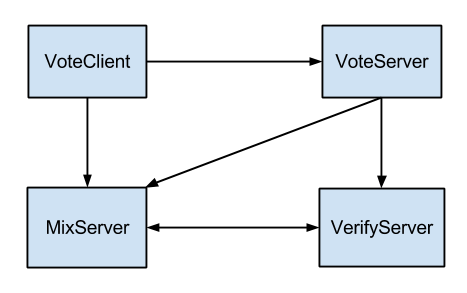
\includegraphics[width=0.8\textwidth]{Comm_diagram.png}
\end{figure}

\section{Libraries}
The mix-net library and voting application will both be written in Java 1.7. For cryptography the Java Cryptography Extension\cite{6}  will be used. Java RMI\cite{7} will be used for setting up communications between the mix servers, the registry server and the clients. JUnit 4\cite{8} is used for unit testing the core classes and applications. A lightweight Java JSON library\cite{9} is used to parse JSON config files .

\section{General Architecture}
The mix-servers will decrypt and shuffle the collection during different stages of the protocol. The protocol is divided into 5 different layers where each layer represents at least a basic Chaum mixnet and therefore each mix server has a keypair for each layer. The verifiers will verify using different verifications during certain stages of the protocol to ensure that it is followed properly.

The protocol requires communication for mix-server to mix-server as well as mix server to verify server. The Verify servers implement the Observable/Observer pattern to notify each observing mix server of any verification results. This way the input of each mix-server and verify server can customized. E.g. a mix-server can choose to only observe the verify servers that it trusts.

The mix-server pushes the collection of votes to the next mix-server in the sequential chain of mix-servers. If it is the last server in the chain, it assumes that the chain overlaps and it pushes to the first mix server in the chain. Each mix server also pushes collections that it decrypts to the verify servers. Each mix-server also listens back to each verify-server to get the results back for different types of verifications. Additionally, it is assumed that any server used to publish the final results of the vote will get its result from the last mix server in the chain.

Each mix server will also serve as a pull service for its released private and public keys. The public keys will be released as soon as they have been generated, while the private keys are released once they are required for the verification-protocol to continue. Attempting to get the public or private keys before they are released will return null. Any client is able to request keys from a mix server.

The vote server will provide an RMI interface for insert votes and will utilise the RMI interfaces of the verify and the first mix server to push the collection of votes into the mixnet. This will also start the decryption process.

The clients will be basic command line applications and only connect to the vote server to input their encrypted values. They will encrypt the message they wish to send using public keys from the each mix server. These public keys are obtained through the RMI interface provided by the mix servers.

\section{CryptoSystem}

The encryption of each message is handled by a CryptoMessage class. The CryptoMessage class takes a message and stores it internally as an array of bytes. It supports operations to add layers or remove layers of encryption where each layer is added or removed using a RSA keypair. To encrypt, an RSA public key is used and thus to decrypt the corresponding private key has to be used.

Under the hood, when adding a new encryption layer, the CryptoMessage first generates a AES key and a byte array seed. It then encrypts the byte array message and the seed using the new AES key and then encrypts the AES key using the passed RSA public key. The now encrypted AES key as well as seed are pushed on top of a stack. This stack represents the encryption layers of the CryptoMessage and can theoretically contain any number of layers.

In order to decrypt, the reverse order of the corresponding RSA private keys are needed. E.g A CryptoMessage encrypted in order using keys Pub1, Pub2, Pub3 will have to be decrypted in the order of Priv3,Priv2,Priv1 to attain the original plaintext.

When decrypting a layer from the CryptoMessage, it uses the private key to decrypt the topmost AES key on the stack. It then decrypts the topmost seed as well as the byte array encrypted message. If decryption is successful the AES key and the seed are both popped off the stack. In order to enable backwards tracing, which is required for finding culprits, the decrypted AES key and seed are pushed onto a new stack. This is so that the same ciphertext can be attained, which is necessary for the backward tracing operation. However it also effectively removes any further privacy using that AES key/seed combination.

The CryptoMessage class also optionally supports signing the message. It implements the Java Serializable interface and can thus be sent over the network.

A subclass of CryptoMessage, ConcatCryptoMessage, exists to concatenate several CryptoMessages into one combined encrypted message. It does this by acting as a container class for the CryptoMessages it will concatenate and using the same AES key and seed to encrypt each of the aforementioned concatenated messages with. Thus decrypting handles much like the original superclass CryptoMessage. The ConcatCryptoMessage class also has a split method which returns the original concatenated messages if and only if no encryption layers are present on top of the ConcatCryptoMessage.

Using the CryptoMessage and ConcatCryptoMessage classes we can now create specific chains of encryptions that can fork and merge.

Additional classes that make up the core cryptosystem are described briefly:
\begin{enumerate}
	\item  CryptoMessageCollection: A simple Serializable collection of CryptoMessages with methods that decrypt, encrypt or sign all messages contained within.
	\item  CryptoHistory and CryptoHistoryItem: Classes that represents a recorded chain of decryptions. Works like a linked list, where each CryptoHistoryItem is a node and references to the next and previous items. The CryptoHistoryItem can verify, using a RSA keypair, that a decryption from one CryptoMessageCollection to another CryptoMessageCollection has been performed properly.
	\item  Verification and VerificationResult: Interface and simple class used to implement different kinds of verifications.
	\item  ExplicitVerification: A class which verifies a chain of CryptoHistoryItems and returns a VerificationResult based on the verification.
  	\item  DummyVerification: A class which creates dummy messages which work as "trip wires" and verifies that they exist in a certain CryptoMessageCollection. If not, they should be traced back to find the culprit, but this has not been implemented yet. 
	\item  TracingVerification: A class which checks so that each message contains exactly T number of messages at the FINAL decryption stage of the protocol. On a failed verification it should then trace back the faulty messages to determine the culprit, but this has not yet been implemented.
\end{enumerate}

\section{Voting Client}

The voting client application is a simple application used to insert votes to the VoteServer. The simple version supplied with the project takes a message to vote for either as a program argument or from STDIN. The client loads its settings from a JSON-formatted file containing the addresses for the VoteServer and Mixservers. It then connects to each of the mixserver and gets each of the mixservers’ public RSA keys. The following diagram describes how the message is encrypted before being sent to the vote server using t=3 repetitions.

\newpage
\begin{figure}
\centering
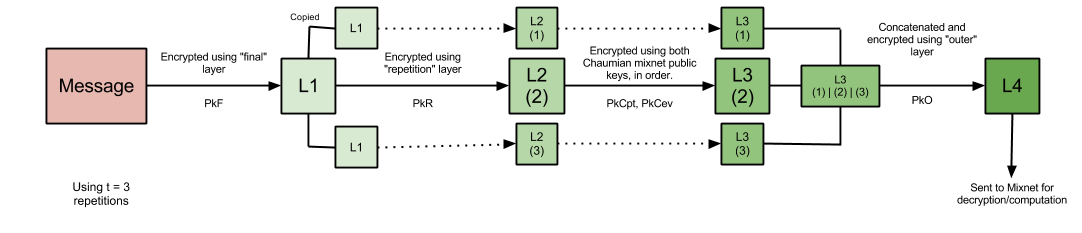
\includegraphics[width=1.0\textwidth]{Sender_Encryption.png}
\end{figure}


Using the CryptoMessage class, the voting plaintext is first encrypted using the FINAL public key for each mixserver in reverse order. It is then cloned into three identical messages and each message is separately encrypted using the REPETITION, MIX1 and MIX2 public keys in the same way as the FINAL encryption layer, that is by encrypting using each mixserver’s public key for the layer. After having added the REPETITION and MIX-layers the messages should contain different ciphertexts but yield the same plaintext once decrypted. The cloned messages are concatenated using ConcatCryptoMessage and finally encrypted using the OUTER layer before being sent to the VoteServer through a Java RMI interface.

It should be noted that no authentication is implemented. In a real world scenario you would most likely expect some sort of authentication to ensure a premise such as each voter only getting one vote.

\section{Vote Server}

The vote servers function is simple. It receives votes from one or more Voter Clients in the form of encrypted CryptoMessages, which it adds to a CryptoMessageCollection. Once the vote is finished it sends the collection of votes to the first mixserver in the mix-net. The state of the vote is controlled by the VoteServer, reading a new line from STDIN closes the vote. In general, the VoteServer has a lot of control over the security of the Vote. It is meant to be a simple application to demonstrate sending input to the mix-net, rather than a secure voting server.

\section{Mix Server}

The main role of the mixserver is to decrypt one or more layers of encryption of CryptoMessages which are sent to it. It publishes its public keys for the clients to use, but keeps its private keys secret until after the decryption is finished.  Using more than one mixserver we can divide up the responsibility of keeping the votes secure and anonymous, so long as the majority are trustworthy.

Each mixserver follows a strict protocol. It receives a CryptoMessageCollection, decrypts it and then sends it to the next mixserver and each of the verifiers. Depending on the current state of the decryption, it waits for result from the verifiers to see if it should continue or not. If it fails to decrypt any CryptoMessage it removes it from the collection. The operations of a mixserver are as follows:

\begin{framed}
\begin{enumerate}
   \item Generate RSA keypairs for each encryption layer. Publish public keys.
   \item  Register self as listener on each of the verifiers.
   \item     Decrypt OUTER layer. If the mixserver is the first in the chain, split the ConcatCryptoMessage into the T duplicates contained within.
   \item     Decrypt MIX1 layer and shuffle the collection.
   \item     Decrypt MIX2 layer and shuffle the collection. Do not send decrypted collection to verifiers.
   \item     Publish private keys used for OUTER and MIX1 layers.
   \item     Wait for Explicit verification of OUTER and MIX1 layer decryptions, stop on failed verification.
   \item     Decrypt REPETITION layer.
   \item     Wait for Tracing verification, stop on failed verification.
   \item     If the mixserver is the last in the chain, group CryptoMessages which have the same ciphertext and remove those which do not have exactly T in count. Save the unique values of cipher texts as the new collection.
   \item     Wait for Dummy verification. If verification fails, stop. Otherwise wait for dummy messages to be published by the verifiers. If the mixserver is the first in the mix-net chain, remove the dummy messages from the collection.
   \item     Decrypt FINAL layer and publish private key used.
   \item     Optionally wait for Explicit verification of FINAL layer decryptions. 
\end{enumerate}
\end{framed}
\begin{center}
Mix Server Protocol
\end{center}

Each mixserver acts a Java RMI server and has an interface for clients to put a CryptoMessageCollection as well as get a KeyCollection of published private or public keys. Using this interface the VoterClients grabs the public keys for encryption, each mixservers passes the current CryptoMessageCollection to the next mixserver and each verifier fetches private keys used for Explicit verifications.

In the current implementation the last mixserver is also responsible for publishing the result of the vote, which it does by just printing it in its terminal. 

\section{Verify Server}

The verify server’s purpose is to verify that each mixserver and voter behaves accordingly. It acts as a Java RMI server and provides an interface for any client to register as a listener callback interface. It uses three different kinds of verification: Explicit, Dummy and Tracing.

Explicit verification takes a chain of CryptoMessageCollections and verifies a subset of these by attempting to perform the same operations as that the mixserver should have performed. If the decryption of each CryptoMessageCollection’s content matches that of the previous CryptoMessageCollection’s, that step of the chain is considered verified. If it does not, the mixserver responsible for that decryption has likely tampered with the collection and has to be reported. However, due to the fact that the verification is separated from the mix operations, it is possible that a mixserver has sent the correct CryptoMessageCollection to the verifier while sending a tampered version to the next mixserver. Perhaps in an effort to frame the next mixserver as a bad one. Thus we can not assume that the mixserver that decrypted it is at fault. This inconsistency could be prevented by adding a synchronization step between the receiving mixserver and the receiving verifiers. This is costly, nearly doubling the amount of traffic sent by each mixserver to the verifiers. Each collection would also have to be signed, so that a mixserver does not try to frame the mixserver it is receiving the collection from.

Dummy verification works by adding a faked Dummy message to the CryptoMessageCollection during the vote and then verifying that the message still exists in the decrypted collection at at certain step.This way we can trap mixservers attempting to replace the entire collection of votes in the MIX2 layer. The vote is inserted through the VoteServer, the same way as a VoteClient would add a vote.

Tracing verification is performed before the FINAL decryption layer is removed. It verifies by making sure there are exactly 3 copies of each ciphertext in the collection. If there is not, either a voter has submitted an incorrect vote or a mixserver has tampered with the vote. In the original protocol definition, this verification is performed more thoroughly by first tracing backwards to find the duplicate ciphertexts and then tracing each duplicate forward again. This way we could find out if it was a mixserver or a voter misbehaving, however due to time constraints it was not implemented.

The protocol of the verify server is tied in directly to that of the mixserver. Its operations are as follows:
\begin{framed}
\begin{enumerate}
	\item  Send dummy vote to the VoteServer.
	\item  Wait until encryption layer MIX2 is decrypted.
	\item  Verify using Explicit Verification that the OUTER and MIX1 layer was decrypted properly. Publish results to any listeners.
	\item  Wait until encryption layer REPETITION is decrypted
	\item Verify using Dummy Verification. Check so that dummy vote is still in the latest collection. Publish results and dummy message to any listeners.
	\item Verify using Tracing Verification that there are T copies of each unique ciphertext. Publish results to any listeners. 
\end{enumerate}
\end{framed}
\begin{center}
Verify Server Protocol
\end{center}

\chapter{Performance / Results}
As a test to evaluate performance, the time taken for different sized mix-nets to decrypt a collection of varied sizes was measured. Time was measured from the closing of the vote to when the result was published. The time taken to insert the votes was excluded. Tests were only performed using servers running on the same machine, running the servers over the network will likely take a longer time. The machine on which the tests were run has a 2.0Ghz Quadcore with Hyperthreading (Intel i7 2630QM) with 8 Gb DDR3 RAM. The tests were run in a virtual machine running Crunchbang (linux).

With a 3 mix server and 3 verify server mix-net and input of 1000 votes with 2 repetitions it took around 70 seconds for the mix-net to process the collection to plaintext. Using the same settings, but without any verify servers, the mix-net was able to decrypt the collection in about 40 seconds.

The current project implementation has the features of the functionality “mix-net with Abort” described in the report by Khazaei, Moran and Wikström \cite{4}. It has limited functionality to determine the culprit, but is able to abort the decryption if it detects tampering.

\chapter{Discussion}
The brief performance test shows that the mix-net implementation is functional and is able to decrypt the votes in a fast enough. As expected, not using any verification speeds up the decryption but not by as much as I initially thought. However, turning of verification means that mix servers and senders can quite easily get away with corrupting the votes.

Compared to the original Helios implementation the performance at this point is decent. In an experiment running Helios on a significantly slower machine in 2008 with 500 votes it was able to obtain results within a few minutes, which one could assume would run faster today. However, this does not take into account the time needed to generate the decryption and shuffling proof, which took several hours \cite{10}. Compared to this implementation the auditing of Helios takes a significantly longer time. However, I am certain that my verifications do not hold the same quality of that of Helios and it should be mentioned that Helios has different features to this, such as open-auditing which lets a voter track their vote. In general it should be stressed that the Helios system is a fully working application and as such comparing it with my limited implementation can be misleading.
\section{Issues and Vulnerabilities}
The biggest issue of the implementation is currently the lack of authentication and input validation. In the mix-net no authentication between mix server or verify servers is performed, each mix- and verify server waits for input which essentially could come from anyone. Obviously this is a pretty big security risk and should be fixed before considering this for any practical use. One simple way to do this would be to add some sort of unique token hash for every user. It is possible that some interfaces could be blocked using a firewall, which would negate the need of authentication in some places. 

The decision to separate the Verification functionality from the Mix server has the downside of adding a window of opportunity for mix-server to "frame" each other. If a mix-server sends a correct version of the vote collection to the verify servers and a corrupt version to the next mix-server in line, the next mix-server will still decrypt the corrupt collection and therefore be blamed when one of the verifications fail. In order to prevent this some sort of synchronization could be implemented to compare vote collections received and/or sent between the mix-servers in question and the verify servers. One way to do this without requiring synchronization with every verifier would be to have each mix-server load a separate subset list of trusted verifiers at startup. Then that mix-server would only trust the output from those verifiers, while still sending decryption results to all of the other verifiers. Using only one trusted verifier hosted on the same server as the mix-server would mimic the behaviour of the original protocol.

It also has to be mentioned that the implementation is far from a complete version of the Khazaei, Moran and Wikström protocol. The original intention was to implement the whole protocol, but due to time constraints certain parts were left unfinished. Primarily the error tracing is missing, which means that in the event of a missing or extra duplicate the implementation will not be able to track down where the corruption originated from. Additionally, there is no guarantee that the cryptosystem implemented in this project is CCA2 secure, which is one of the main selling points as to say of their report. However, the CryptoMessage class is likely not that difficult to modify so that it uses an algorithm to encrypt and decrypt in a CCA2 secure manner. All encryption is abstracted to the CryptoMessage class, thus probably making necessary modifications relatively easy.

The system is also very easy to obstruct using a Denial of Service attack. A mix or verify server can simply chose to not partake in the decryption, effectively wasting the entire vote. In this case it is easy to determine who the culprit is however.

Performance-wise the protocol can be improved by pipelining the decryption of individual CryptoMessages instead of whole collections. This way two mixservers and even verifiers can work in parallel, decrypting messages at the same time instead of the current sequential implementation where each mixserver decrypts each of the message in the collection. The only layer of encryption where the sequential decryption is necessary is the MIX2 layer, because of the shuffle operation performed to hide the source of the vote, so a predicted ~80\% of the decryption process could be sped up using a parallel pipeline. At the same time, time measurements were not taken of failing mixnet decryptions. I.e. decryption processes where a mix-server tries to manipulate the ballot were measured by time. 

\chapter{Conclusion}
The protocol desbired by Khazaei, Moran and Wikström is partly implemented in Java for a voting system with features to prevent  The implementation described in this report should be considered as an example application rather than something to be used in a real election. 
Still, it performs reasonably efficiently and can be seen as the beginning of something greater. With some modifications, such as adding authentication between the different components and a full implementation of the error tracing described in the original protocol it could perhaps be seen as a relatively secure electronic voting system. 
If you are interested in the code, it is available under the GNU General Public License at \url{https://github.com/Tethik/mixnet}

\begin{thebibliography}{12}
\bibitem{1}
 “Untraceable electronic mail, return addresses, and digital pseudonyms” - David L. Chaum, University of California, Berkeley. Feb 1981
 \url{https://mirror.robert-marquardt.com/anonbib/cache/chaum-mix.pdf}
\bibitem{2} 
Tor project: Anonymity Online. 
\url{ https://www.torproject.org/}
\bibitem{3}
 Bitcoin Fog Company.
 \url{http://www.bitcoinfog.com/}
\bibitem{4}
 “A Mix-Net From Any CCA2 Secure Cryptosystem” - Shahram Khazaei, Tal Moran, Douglas Wikström.
 \url {http://www.csc.kth.se/~dog/research/}
\bibitem{5} 
 “The Black Box Report: SECURITY ALERT: July 4, 2005 Critical Security Issues with Diebold Optical Scan Design” - Harri Husti.
 \url{http://www.blackboxvoting.org/BBVreport.pdf}
\bibitem{6}  
“Java Cryptography Extension”, 2013-04-11
 \url{http://docs.oracle.com/javase/1.4.2/docs/guide/security/jce/JCERefGuide.html}
\bibitem{7} 
"Remote Method Invocation", 2013-04-11 
\url{http://www.oracle.com/technetwork/java/javase/tech/index-jsp-136424.html}
\bibitem{8}
 JUnit - Java Unit testing framework, 2013-04-11 
\url{http://junit.org/}
\bibitem{9} 
Java JSON library, 2013-04-11 
\url{https://github.com/Tethik/JSON-java}
\bibitem{10} 
“Helios: Web-based Open-Audit Voting” -  Ben Adida, 2008-09-19 
\url{http://static.usenix.org/events/sec08/tech/full_papers/adida/adida.pdf}
\bibitem{11}
 Scantegrity,  2013-04-12
\url{http://scantegrity.org/}
\bibitem{12}
"The Prêt à Voter Verifiable Election System" - Peter Y. A. Ryan, David Bismark, James Heather, Steve Schneider, Zhe Xia. University of Luxembourg, University of Surrey 
\url{http://www.pretavoter.com/publications/PretaVoter2010.pdf}
\end{thebibliography}

% \appendix
% \addappheadtotoc
% \chapter{RDF}\label{appA}

%\begin{figure}[ht]
%\begin{center}
%And here is a figure
%\caption{\small{Several statements describing the same resource.}}\label{RDF_4}
%\end{center}
%\end{figure}

%that we refer to here: \ref{RDF_4}
\end{document}
